%!TEX root = ../dissertation.tex

\chapter{Evaluation}
\label{chapter:evaluation}




\section{GD capability}
The goal of our work was to bring \gls{gd} to the web browser so it can be used anywhere more easily.
To do this, we implemented a set of primitives that produce several 3D concepts to be used as building blocks for modeling.

Now comes the time to test the environment's ability to be used for \gls{gd}, more specifically to produce diverse 3D models.
In order to evaluate this, we developed several programs that reproduce examples that were previously done in other \gls{gd} environments.
The results of these programs are shown in Figure \ref{fig:all:examples}.

\begin{figure}
  \centering
  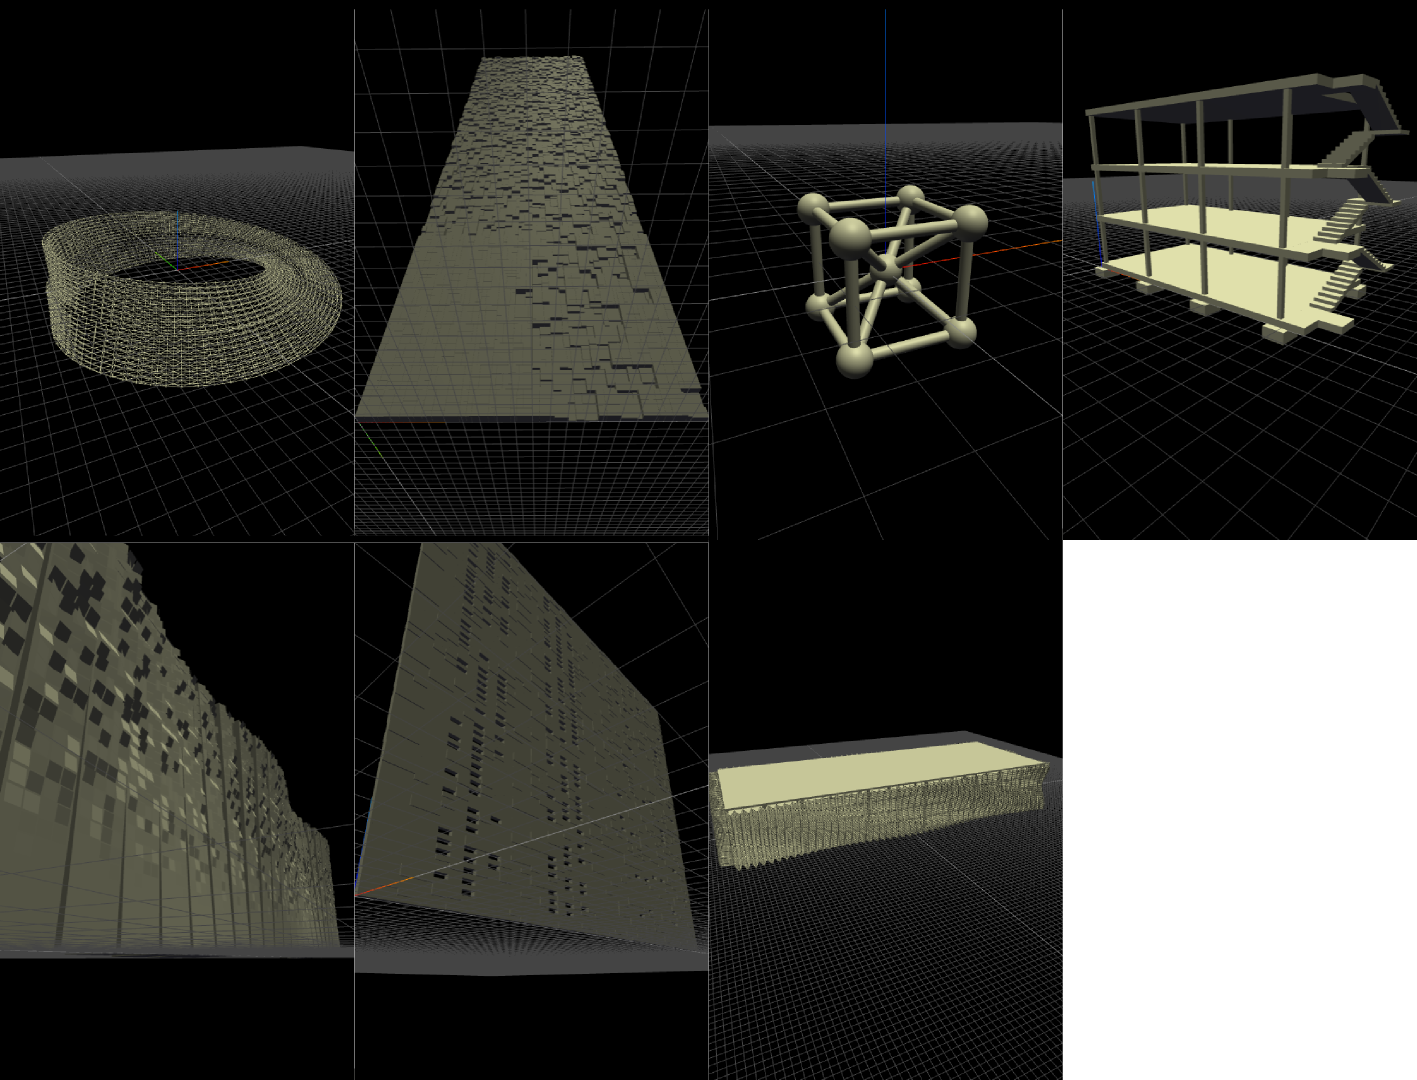
\includegraphics[width=12cm]{./images/all_examples}
  \caption{Renderings of results of the implemented example programs.}
  \label{fig:all:examples}
\end{figure}

As shown, the environment can produce interesting results with varying degrees of complexity.
The range of results is still limited by the primitives currently implemented.
None of these examples make use of \gls{csg} operations like union, intersection and difference as these were not implemented.
Nevertheless, it is clearly possible to add support for these without major effort since there are already JavaScript implementations of \gls{csg}, like the case of OpenJSCAD's.


\section{Real Use}
{\it This is where I give the prototype to an architect, ask him to do a building, get his feedback, and tell it to the world.}


\section{Performance}
There are several areas where performance plays an important part when using the environment.


\subsection{Running Performance}
Running performance is a prevalent part of programming in \gls{gd} since it dictates the complexity of the programs that can be explored interactively.

After a program as become too complex, hence too slow, it can no longer be tested as a whole.
So, it needs to be split into smaller parts that are still fast enough to be explored interactively.

To see how the performance of our web-based \gls{gd} environment compares to the existing environments, we compared the time each takes to generate identical models.
First, we implemented different versions of the program in each of the environments and, then, measured the time each took to complete.
The times can be seen in Figure \ref{fig:run:timing:chart}.

We compared our environment with Rosetta (using the OpenGL backend), OpenJSCAD and Rhino+Grasshopper.

\begin{figure}
  \centering
  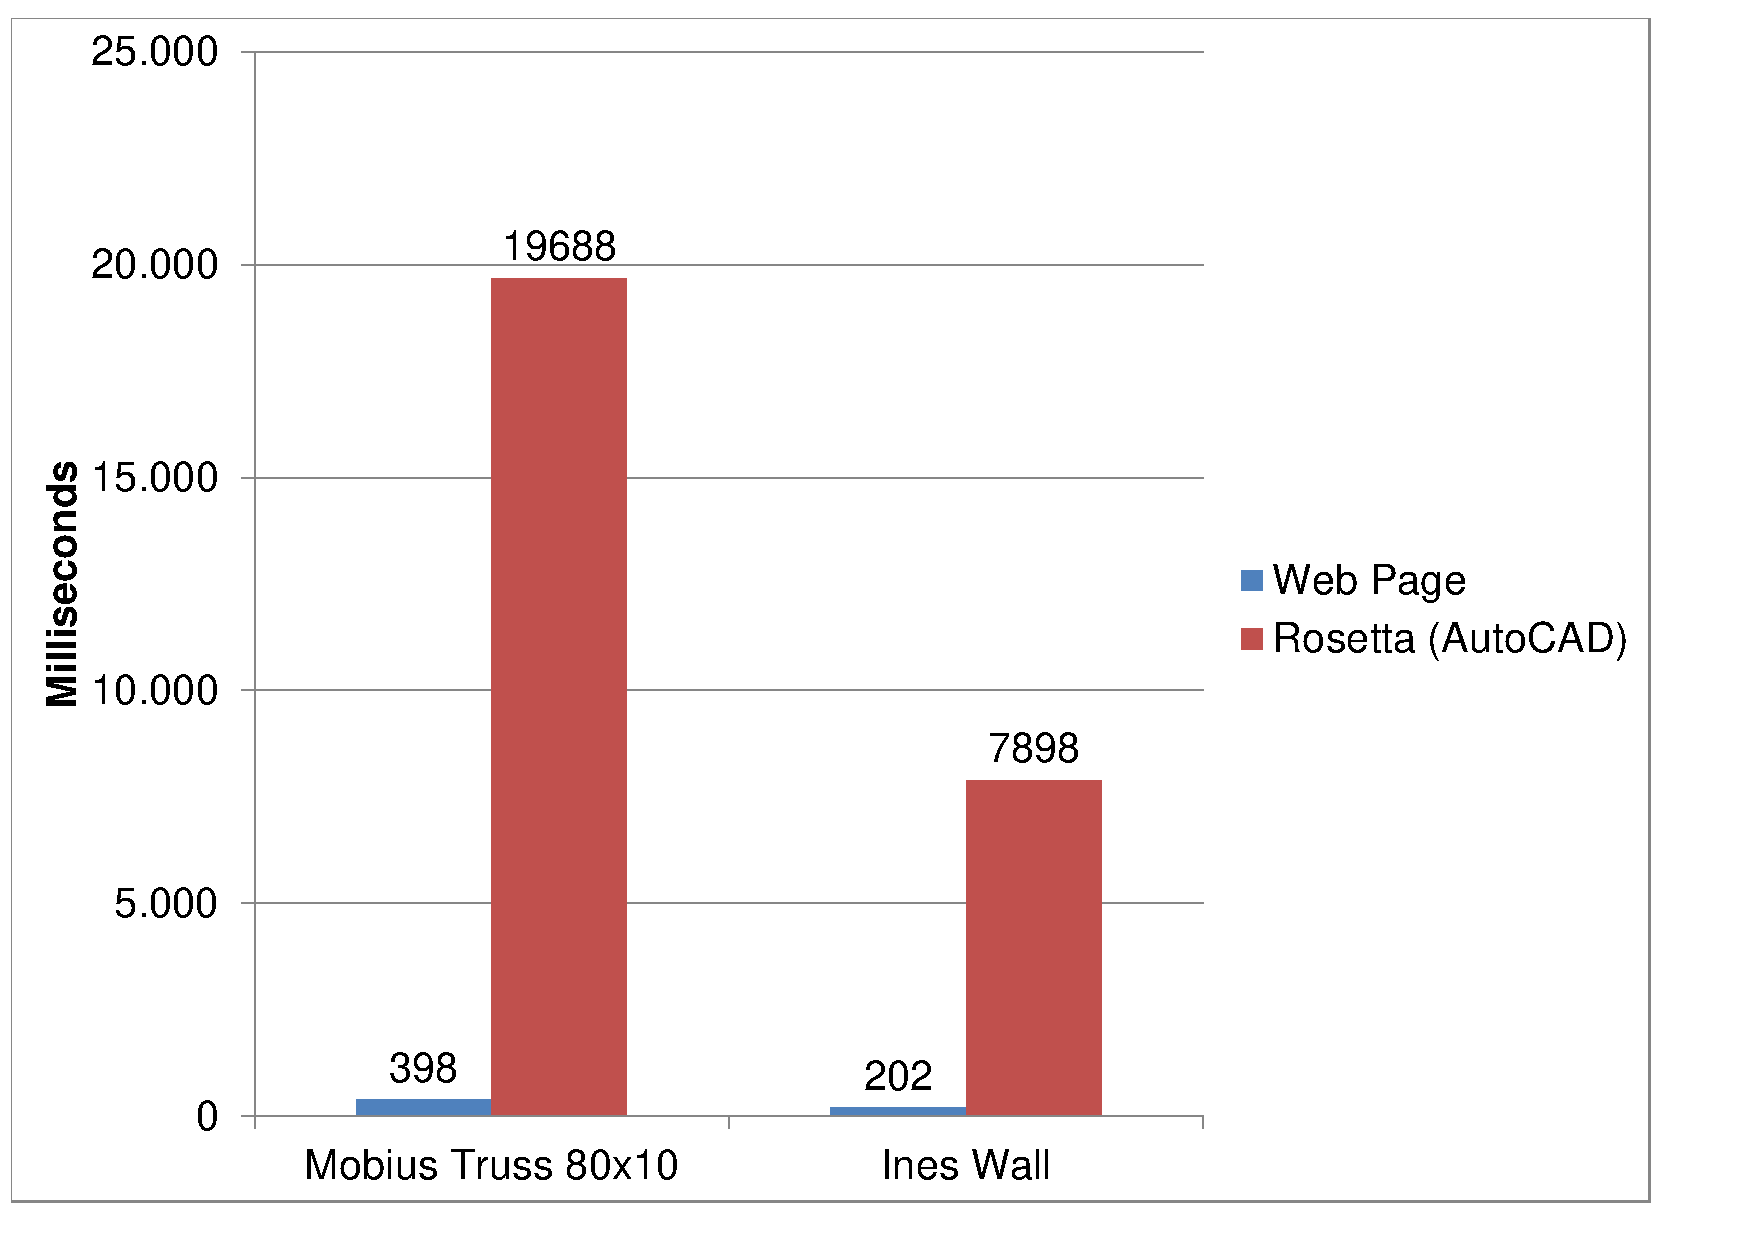
\includegraphics[width=12cm]{./images/run_timing_chart}
  \caption{Running times for completing the generation of the test model.}
  \label{fig:run:timing:chart}
\end{figure}

Observations, observations, observations.

All of them ran in the same computer.
{\it Insert hardware specs.}

The source code of each program used in the test is available at ABC (either here, appendix or github).


\subsection{Export Performance}
When time comes to pass on the building design to other people that use different tools -- like mechanical, electric, plumbing services or even other architects -- the architect must provide it in a format compatible with their tools.
This has been covered in our solution by letting the program that generates the building model run in a \gls{cad} tool.

The next step was to know how the execution time differs between the normal running process and the remote \gls{cad} running process.
To measure the difference, we ran a program of some complexity using both processes and measured the time each took to complete.
The graph in Figure \ref{fig:local:remote:timing} shows their timings and how they compare.

\begin{figure}
  \centering
  
\includegraphics[width=12cm]{./images/local_remote_timing}
  \caption{Running in web page compared to running in a \gls{cad}.}
  \label{fig:local:remote:timing}
\end{figure}

Observations, observations, observations.

Conclusion: Develop in the environment because it's faster. Only ``convert'' when necessary. (as probably already stated)


\subsection{Traceability Performance}
{\it Let us see how keeping track of traceability information influences the time programs take to complete. Measure for programs of different complexity.}

%Describe possible programming techniques using the IDE / our solution.
%- Examples of use (made by me)
%- Example from architect (e.g. Inês Caetano)
%Describe possible use cases using our solution.

%GD capabilities(examples)
%- Architect example
%- More examples
%Performance:
%- web page vs rosetta vs grasshopper/dynamo
%- running in web page vs running in remote CAD service
%- impact of traceability tracking
%Geometry/primitives: our solution vs existing solutions

%Usefulness of traceability?
